\documentclass[10pt]{article}
\title{What I have learnt in Latex so far...}
\author{Bilal Ahmed Khan\thanks{Administration FAST NU}}
\usepackage[utf8]{inputenc}
\usepackage{ulem}
\usepackage{graphicx}
\usepackage{amsmath}
\date{14th January 2020}

\begin{document}
\maketitle
\tableofcontents
\newpage
\section{Bold, italic and underline}
\subsection{Bold}

\noindent\textbf{This text is bold}
\subsection{Italic}

\noindent\textit{This text is italic}
\subsection{Underline}
\subsubsection{Using underline}

\noindent\underline{This text is underlined using underline}
\subsubsection{Using uline}

\uline{This pararaph is underlined using uline. I am using this because underline function usually doesnot work well with multilined text.}
\section{Adding images to a latex report}
\subsection{Adding an image}
\textbf{This is how you add images to a latex report}

\begin{figure}[h!]
    \centering
    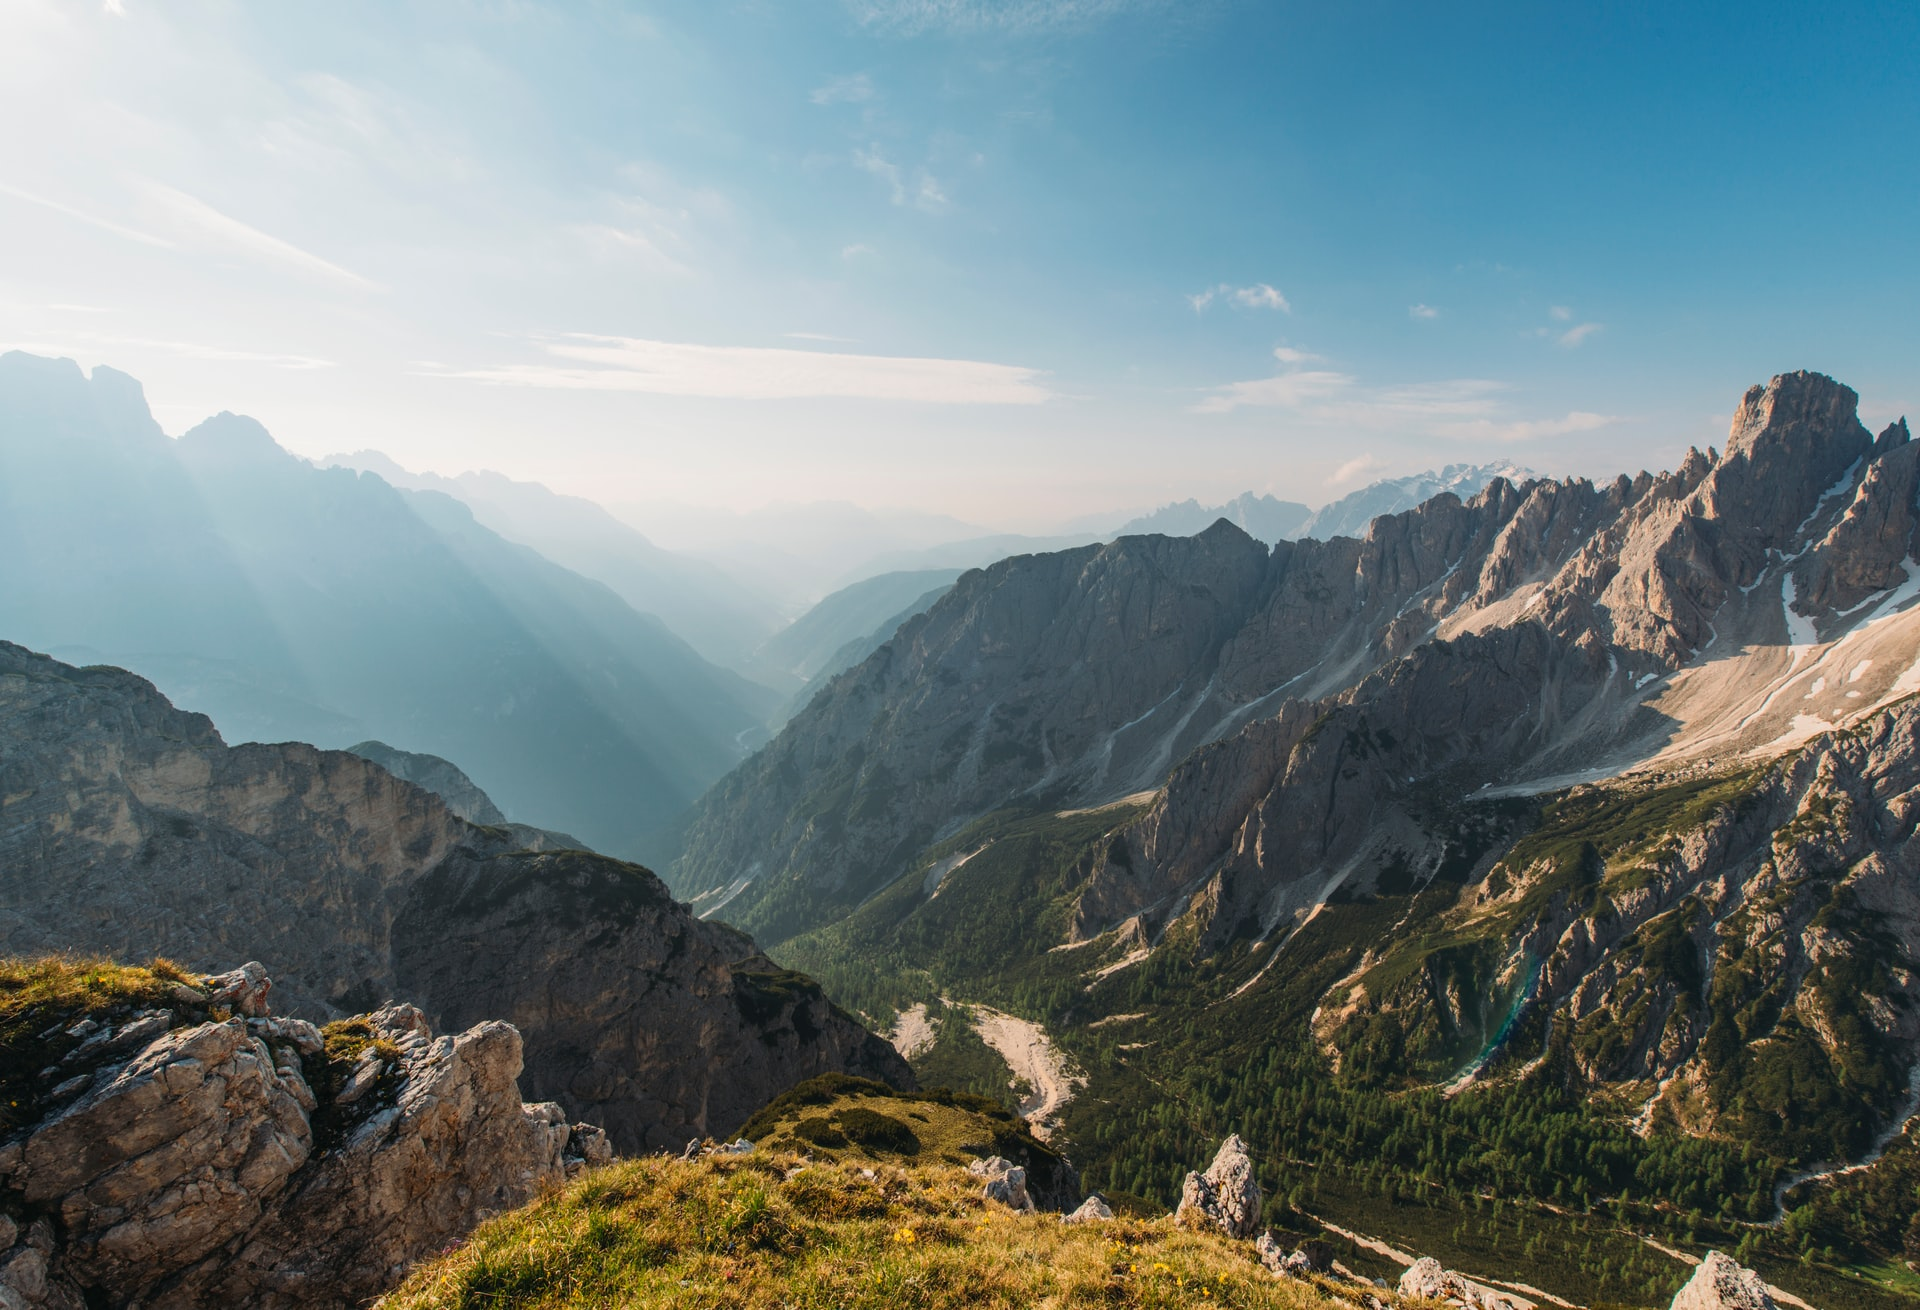
\includegraphics[width =0.5\textwidth]{beautiful mountain pics.jpg}
    \caption{Motivation Wallpaper}
    \label{fig:mountains}
\end{figure}
\subsection{Referencing and Captions}
The wallpaper you see in Figure \ref{fig:mountains} on page number \pageref{fig:mountains} is my \textit{scenery }of all time. It reminds of the \textbf{grandeur} of nature and how \underline{small} we are.

From the next page I'll talk about \textbf{something} else ;).
\newpage
\section{Lists and their types in Latex}
Okay so now lets talk about lists. In \LaTeX  there are 2 kinds of lists.

\begin{enumerate}
    \item Ordered Lists.
    \item Unordered Lists.
\end{enumerate}
\subsection{Unordered Lists}
So now lets talk about \textbf{Unordered Lists}. Here is a list of my new year resolutios.
\begin{itemize}
    \item I'll try to be more punctual
    \item {\large I'll study more}
\end{itemize}
\subsection{Ordered Lists}
Following is the list of my favorite Pakistani Players

\begin{enumerate}
    \item Babar Azam
    \item Shaheen Afridi
    \item Haider Ali
    \item Amad Butt
\end{enumerate}

Form next page I am going to talk about mathematical equations.

\newpage
\section{Various kind of mathematical equations in Latex}
On this page we are gonna talk about Adding math in a report. Mathematical Equations can be added by two methods.
\subsection{Modes of displaying an equation in \LaTeX}
\begin{enumerate}
    \item In line
    \item On display
\end{enumerate}

Firstly, We will talk about \underline{\textbf{In-line} }method of writing mathematical equations

Einstein discovered the relation between light and mass {\large(\(E=mc^2\))} in 1905

This formula can also be written as\[m=E/c^2\]\
In natural units \(c=1\), Hence we can also write
{\Large
\begin{align*}
    \nonumber
    E&=mc^2  \\
    \nonumber
    E&=m(1)\\
    E&=m
\end{align*}
}
\subsection{Integrals}
integrals can be written like this;

{\large\[\int_0^1\frac{1}{e^x}=\frac{e-1}{e}\]}
\subsection{Trignometic functions}
You can also write trig functions like this 
{\Large\[\sin({\alpha+\beta})=\sin{\alpha}\cos{\beta}+\cos{\alpha}\sin{\beta}\]}

Now lets talk about the sum of a series:
\subsection{Sequence and Series}
{\large\[a_1+a_2+a_3+\dots+a_n=2a+(n-1)d\]}

Where

\begin{flushleft}
    a= first term\\
    n= number of terms\\
    d= arithematic difference between two consecutive terms
\end{flushleft}

The sum of an infinite Geometric series where \(r<1\) is given by:
\begin{align}
S=\frac{a}{1-r}
\end{align}
\subsection{Summation}
You can also write summations like this:
\[\sum_{n=1}^\infty n=\frac{n(n+1)}{2}\]

\subsection{Writing expressions which contain square root}
In \LaTeX you can write a square root like this pythgorean theorem
\begin{equation*}
    H^2=\sqrt{B^2+P^2}
\end{equation*}

\newpage
\section{Paragraphs, abstracts, tables and formatting etc}
\subsection{Abstracts}
\begin{abstract}
    Abstract is a paragraph in the beginning of the page to provide some key information to the reader
\end{abstract}
Form now on we'll talk about formatting latex.
\noindent Let us first talk about Abstract
\subsection{Tables of various types}
Creating \textbf{Tables} in \LaTeX

Following are the tables of me and my uni friends in different styles:
\begin{table}[h!]
\centering
\begin{tabular}{c c c}
     Serial No.& Name & Roll No.  \\
     01 & Bilal Ahmed Khan & 0183 \\
     02 & Wamiq Akram & 1857 \\
     03 & Zulnoor Siddiqui & 1090
\end{tabular}
\caption{Friends in uni}
\end{table}

Now with borders:

\begin{table}[h!]
\centering
\begin{tabular}{|c| c| c|}
    \hline
     Serial No.& Name & Roll No.  \\\hline
     01 & Bilal Ahmed Khan & 0183 \\\hline
     02 & Wamiq Akram & 1857 \\\hline
     03 & Zulnoor Siddiqui & 1090 \\\hline
\end{tabular}
\caption{Friends in uni}
\end{table}

Now with double lines

\begin{table}[h!]
\centering
\begin{tabular}{||c|| c|| c||}
    \hline\hline
     Serial No.& Name & Roll No.  \\\hline\hline
     01 & Bilal Ahmed Khan & 0183 \\\hline\hline
     02 & Wamiq Akram & 1857 \\\hline\hline
     03 & Zulnoor Siddiqui & 1090 \\\hline\hline
\end{tabular}
\caption{Friends in uni}
\end{table}

With gap between each row:

\begin{table}[h!]
\centering
\begin{tabular}{||c ||c|| c||}
    \hline\hline
     Serial No.& Name & Roll No.  \\[2ex]
     \hline\hline 
     01 & Bilal Ahmed Khan & 0183 \\\hline\hline
     02 & Wamiq Akram & 1857 \\\hline\hline
     03 & Zulnoor Siddiqui & 1090 \\\hline\hline
\end{tabular}
\caption{Friends in uni}
\end{table}
\newpage
Copy Paste from manual
\begin{table}[h!]
\centering
\begin{tabular}{||c c c c||}
\hline
Col1 & Col2 & Col2 & Col3 \\ [0.5ex]
\hline\hline
1 & 6 & 87837 & 787 \\
\hline
2 & 7 & 78 & 5415 \\
\hline
3 & 545 & 778 & 7507 \\
\hline
4 & 545 & 18744 & 7560 \\
\hline
5 & 88 & 788 & 6344 \\ [1ex]
\hline
\end{tabular}
\caption{Table to test captions and labels}
\end{table}
\end{document}